% !TEX encoding = UTF-8 Unicode
\documentclass[10pt,aspectratio=169]{beamer} % 169 为4:3比例
\setbeamercovered{transparent=20}
\usetheme[
%  showheader,
%  red,
%  purple,
%  gray,
  lightBlue,
%  colorblocks,
%  noframetitlerule,
]{scnu}

\usepackage[T1]{fontenc}
\usepackage[utf8]{inputenc}
\usepackage{lipsum}
\providecommand{\lishu}{\CJKfamily{song}}
\usepackage{tikz}
\usetikzlibrary{fadings}
%\setbeamertemplate{sections/subsections in toc}[ball]
\usepackage{xeCJK}
\usepackage{listings}
\usepackage{caption}
\usepackage{subcaption}
\usefonttheme{professionalfonts}
\def\mathfamilydefault{\rmdefault}
\usepackage{amsmath}
\usepackage{multirow}
\usepackage{booktabs}
\usepackage{bm}
\setbeamertemplate{section in toc}{\hspace*{1em}\inserttocsectionnumber.~\inserttocsection\par}
\setbeamertemplate{subsection in toc}{\hspace*{2em}\inserttocsectionnumber.\inserttocsubsectionnumber.~\inserttocsubsection\par}
\setbeamerfont{subsection in toc}{size=\large} % 设置目录样式
%---------------------------------------------------------------------
%在章节开始前放映章节目录
\AtBeginSection[]{%
\begin{frame}%
\frametitle{Outline}%
\textbf{\tableofcontents[currentsection]} %
	\end{frame}%
}
%--------------------------------------------------------------------
% 在子章节开始前放映子章节目录
%\AtBeginSubsection[]{%
%	\begin{frame}%
%		\frametitle{Outline}%
%		\textbf{\tableofcontents[currentsection, currentsubsection]} %
%	\end{frame}%
%}
%===================================================================
\title{Title}
\subtitle{}   % 子标题
\author[YuXuan Li]{答辩人:姓名}
%\mail{\large yxli@m.scnu.edu.cn}
\institute[South China Normal University]{\large 专业:凝聚态物理\\指导老师:某某\quad 教授}
\date{\today}
\titlegraphic[width=3cm]{logo_01_scnu}{}  % 在首页显示校徽
%===================================================================
\begin{document}
\maketitle
\begin{frame}%
\frametitle{Outline}%
\textbf{\tableofcontents} %
\end{frame}
%=======================================================
\section{研究背景}
%---------------------------
\begin{frame}
\frametitle{拓扑绝缘体}
\begin{columns}
\column{0.5\textwidth}
\begin{figure}[h]
\flushleft
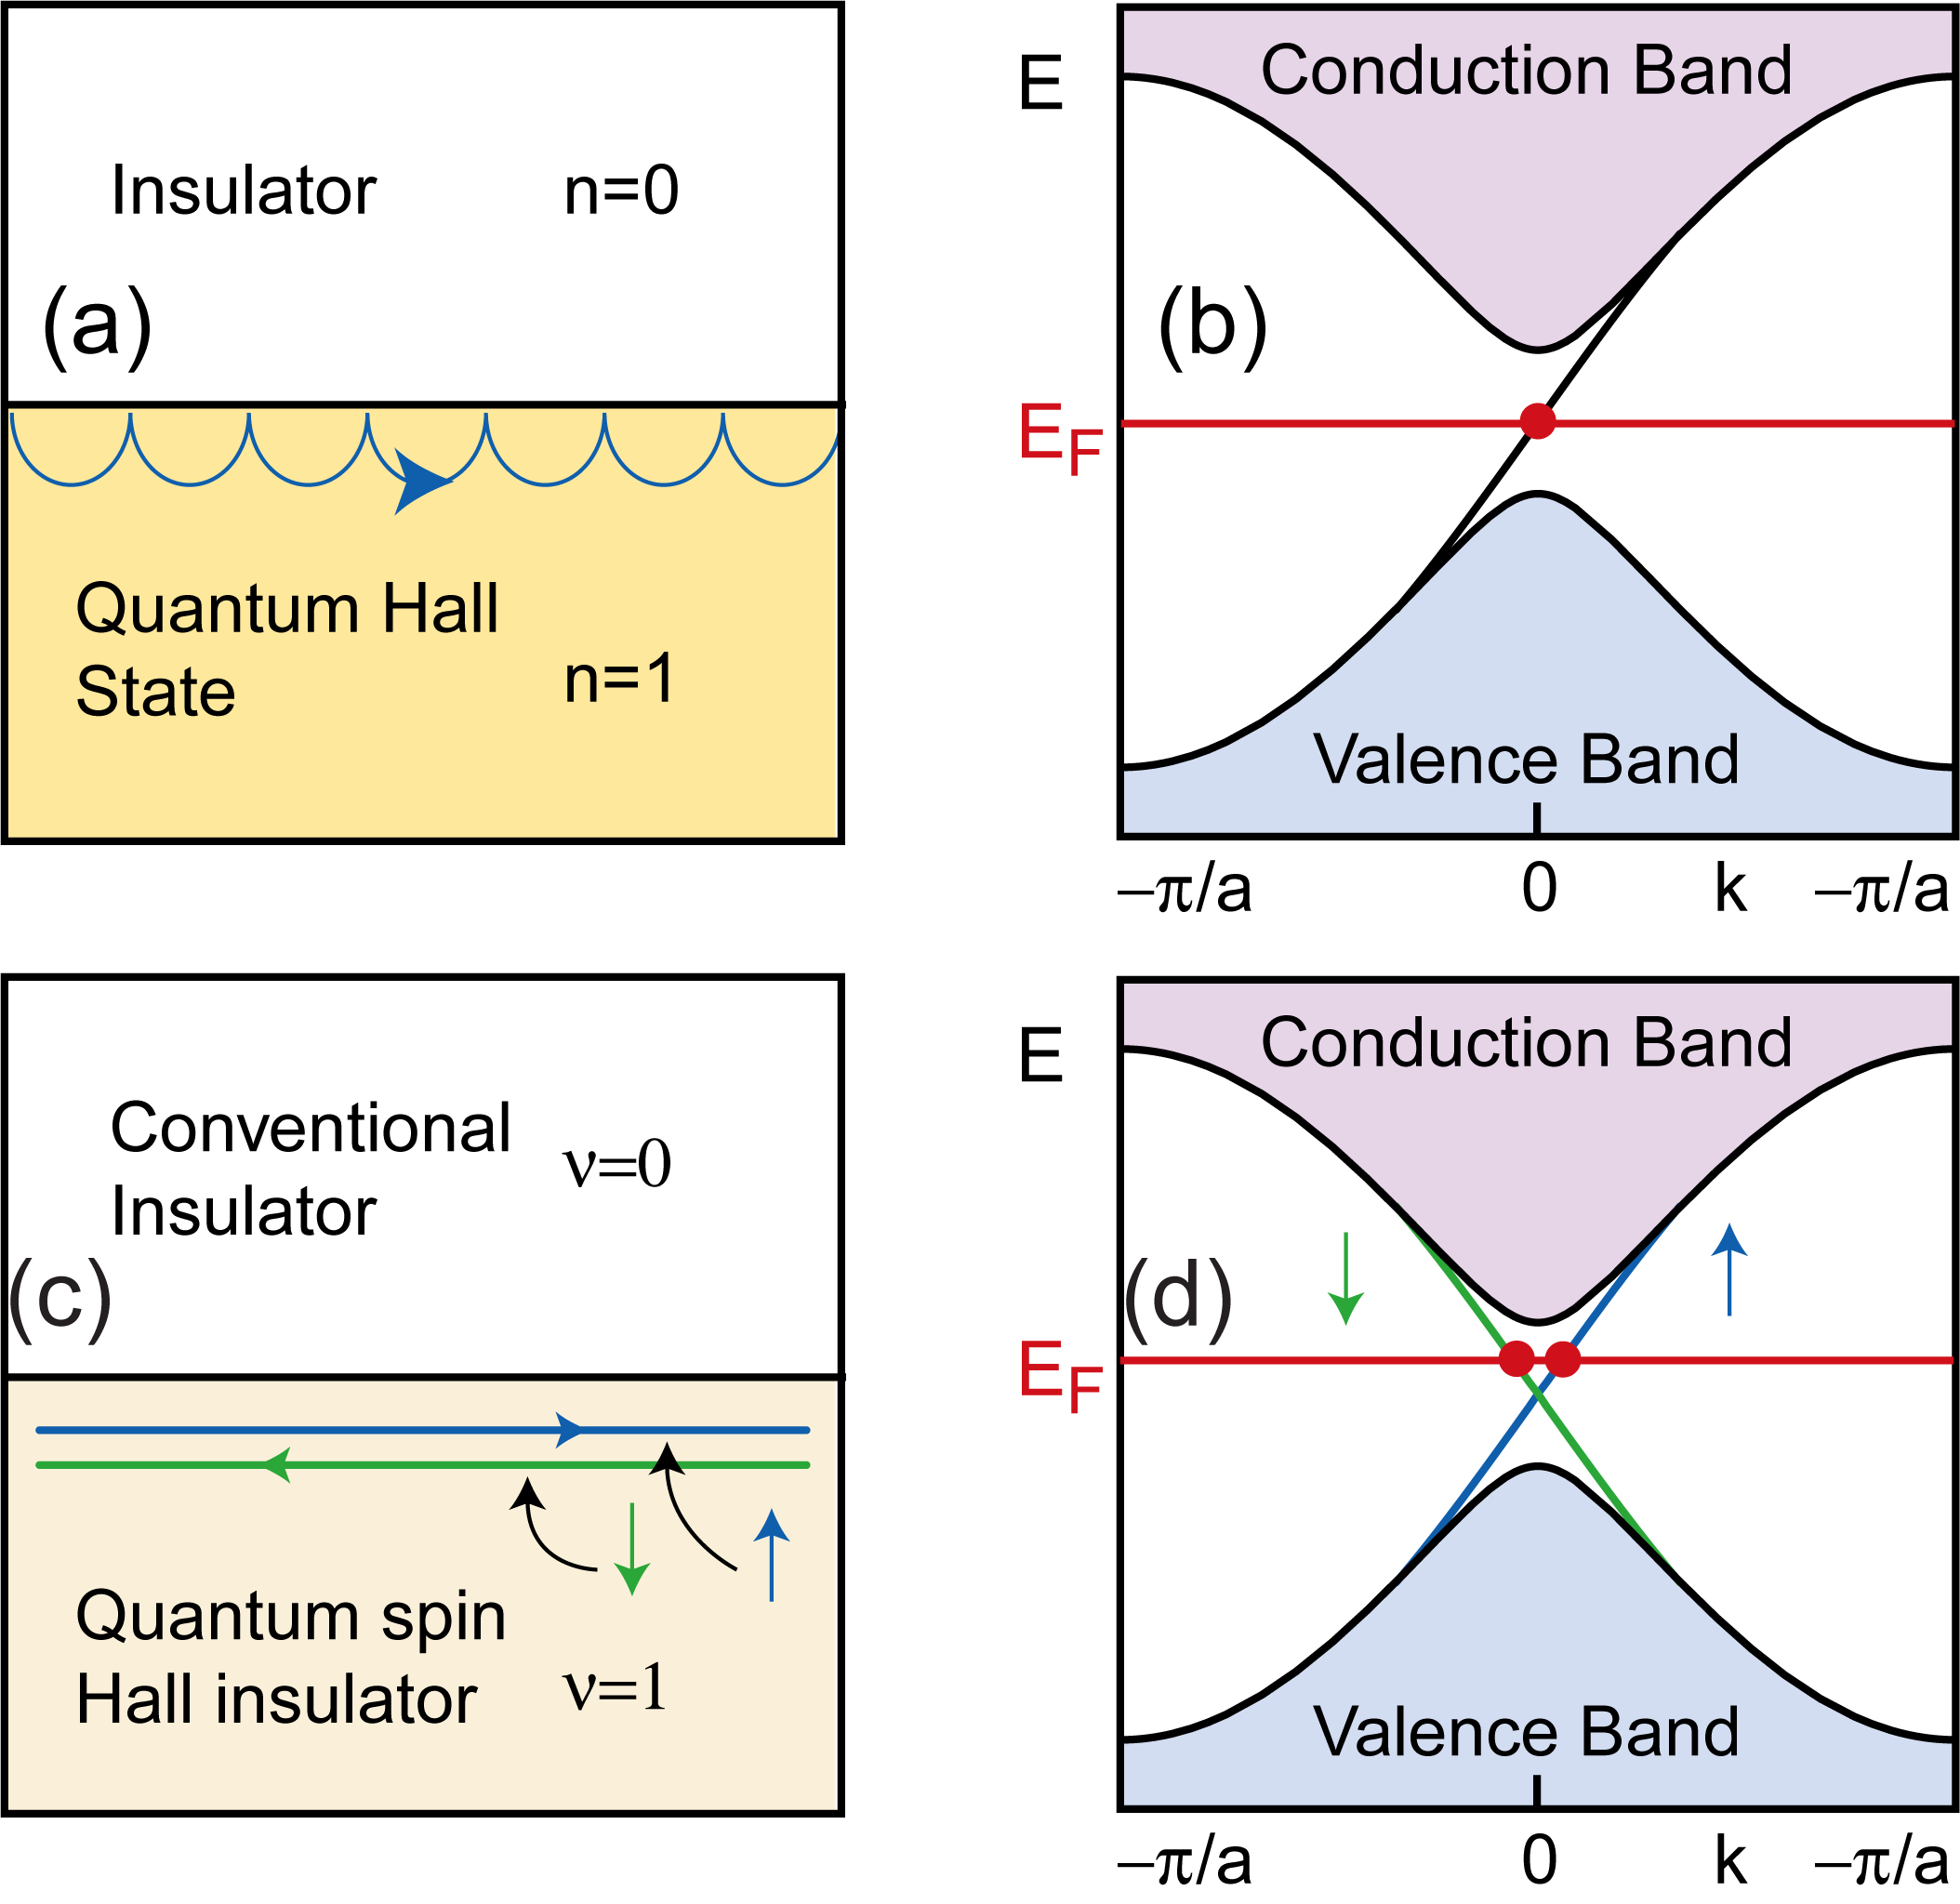
\includegraphics[scale=0.4]{pic/fig1.png}
\end{figure}
\bigskip
\column{0.4\textwidth}
\begin{equation}	
	n=\frac{1}{2}\int_{\mathrm{BZ}}d^2k\nabla_k\times i\sum_{l\in\mathrm{bands}}\langle\varphi_l|\nabla_k|\varphi_l\rangle\label{chern_num}
\end{equation}
\end{columns}
\end{frame}
%---------------------------
\begin{frame}
	\frametitle{高阶拓扑}
	\begin{figure}[h]
		%\flushleft
		\centering
		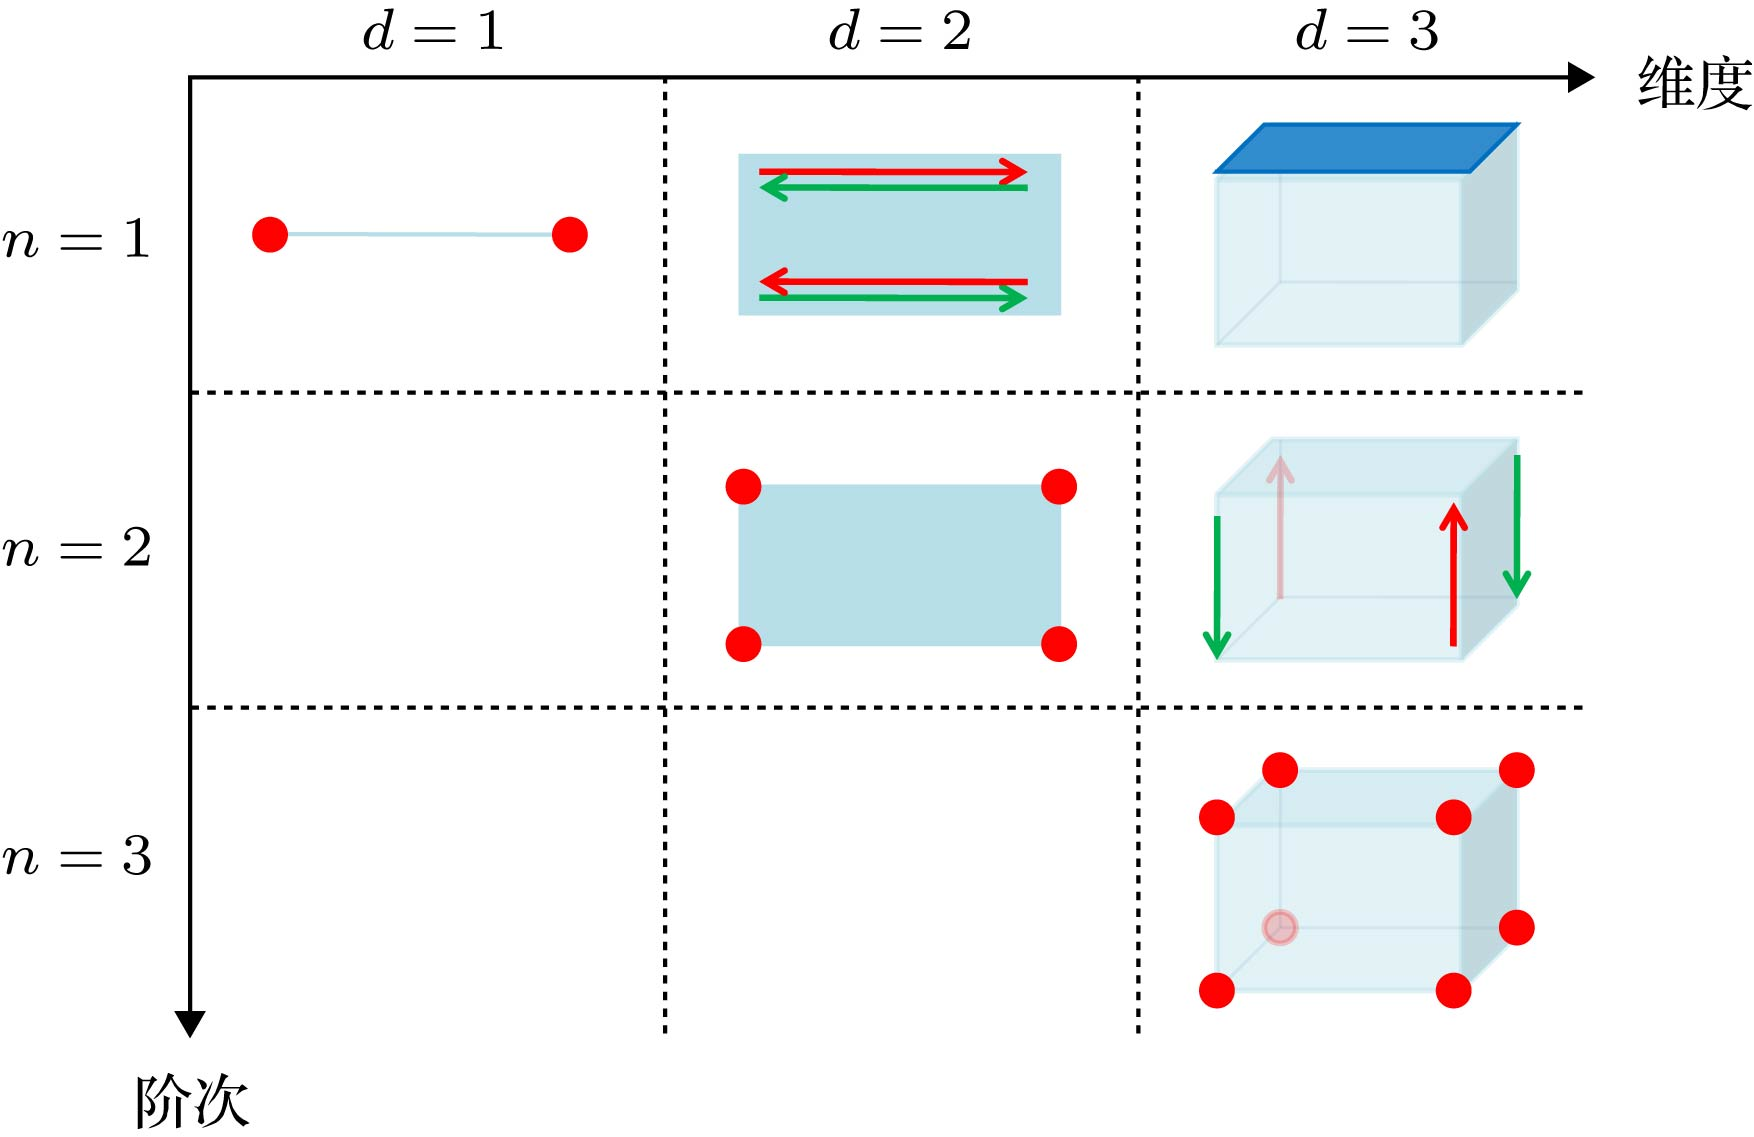
\includegraphics[scale=1.4]{pic/fig6}
	\end{figure}
\end{frame}
%----------------------------------
\begin{frame}
	\frametitle{高阶拓扑绝缘体}
	\begin{equation}
	H_c(\mathbf{k})=(M+t\sum_i\cos k_i)\tau_z\sigma_0+\Delta_1\sum_i\sin k_i\tau_x\sigma_i+\Delta_2(\cos k_x-\cos k_y)\tau_y\sigma_0\label{hoti}
	\end{equation}
	\begin{equation}
	(\hat{C}_4^z\mathcal{T})H_c(\mathbf{k})(\hat{C}_4^z\mathcal{T})^{-1}=H_c(D_{\hat{C}_4^z\mathcal{T}}\mathbf{k}),\quad D_{\hat{C}_4^z\mathcal{T}}\mathbf{k}=(k_y,-k_x,-k_z)
	\end{equation}
	\begin{figure}[h]
		\centering
		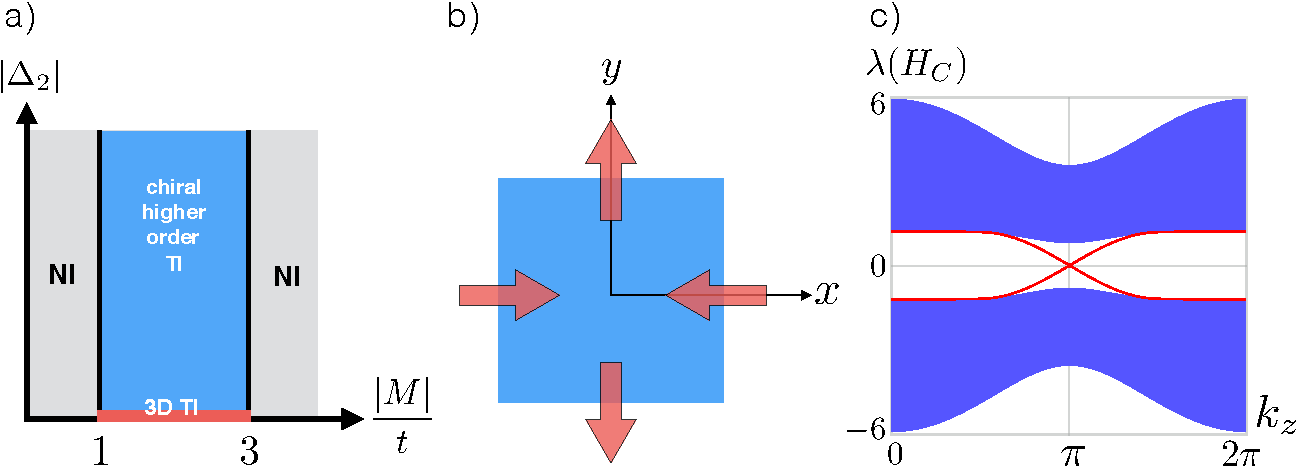
\includegraphics[scale=0.5]{pic/fig7}
		\caption{手性高阶拓扑绝缘体;(a)哈密顿量(\ref{hoti})的相图,(b)一个元胞内满足$\hat{C}_4^z\mathcal{T}$的非共线反铁磁,(c)存在手性棱态(红色)的哈密顿量(\ref{hoti})的能谱图}\label{fig7}
	\end{figure}
\end{frame}
%--------------------------------------------------------------
\begin{frame}{近邻效应}
\begin{figure}[h]
\centering
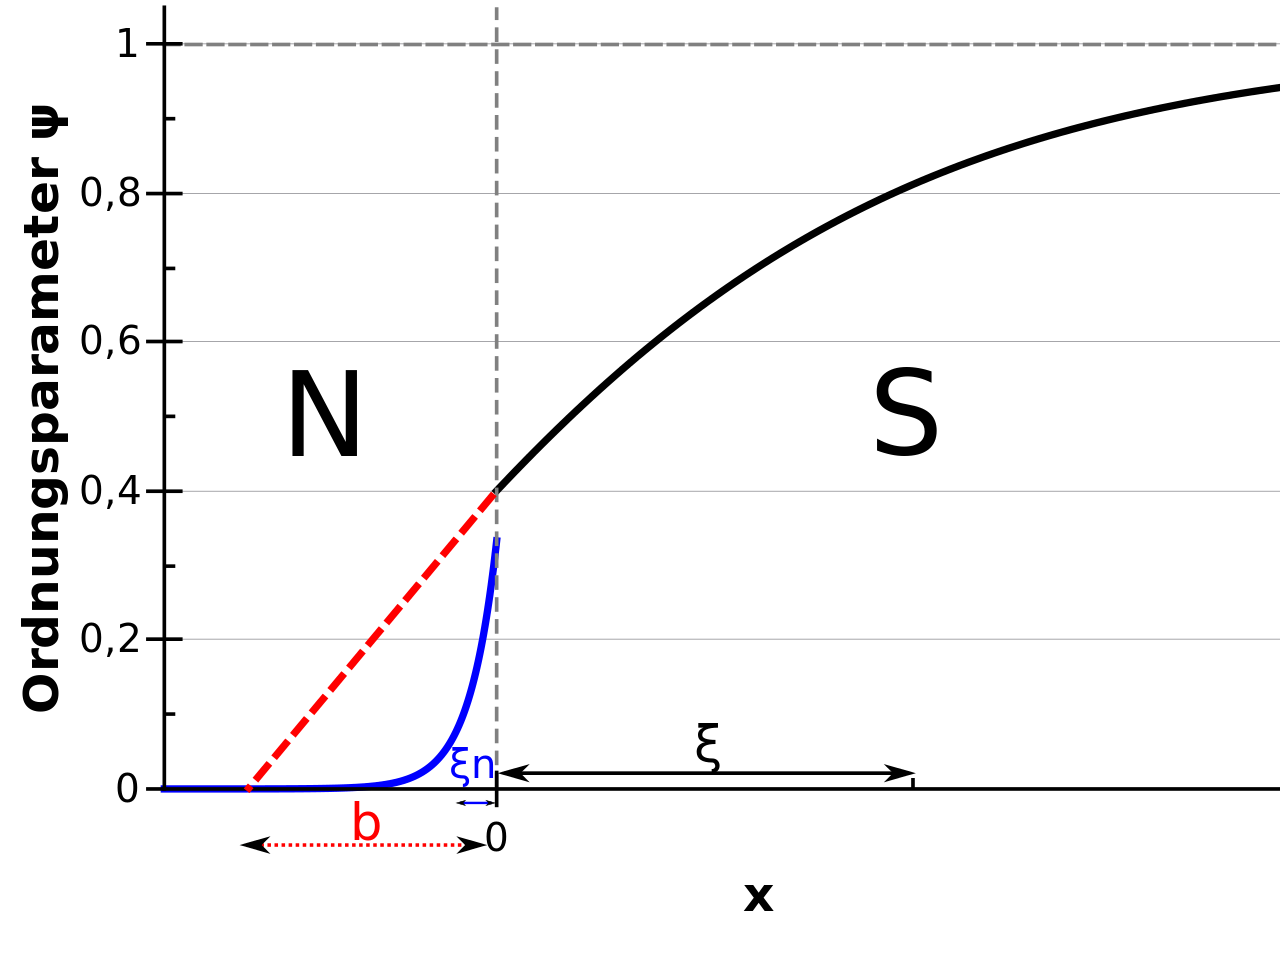
\includegraphics[scale=0.15]{pic/pro}\label{fig5}
\end{figure}	
\end{frame}
%--------------------------------------------------------------
\begin{frame}{高阶拓扑超导体}
\begin{equation}
\begin{aligned}
H(\mathbf{k})&=M(\mathbf{k})\sigma_z\tau_z+A_x\sin k_x\sigma_xs_z+A_y\sin k_y\sigma_y\tau_z+\Delta(\mathbf{k})s_y\tau_y-\mu\tau_z\\
M(\mathbf{k})&=m_0-t_x\cos k_x-t_y\cos k_y\label{hoti2}
\end{aligned}
\end{equation}
\begin{equation}
\Delta(\mathbf{k})=\Delta_x+\Delta_x\cos k_x+\Delta_y\cos k_y
\end{equation}
\begin{figure}[h]
\centering
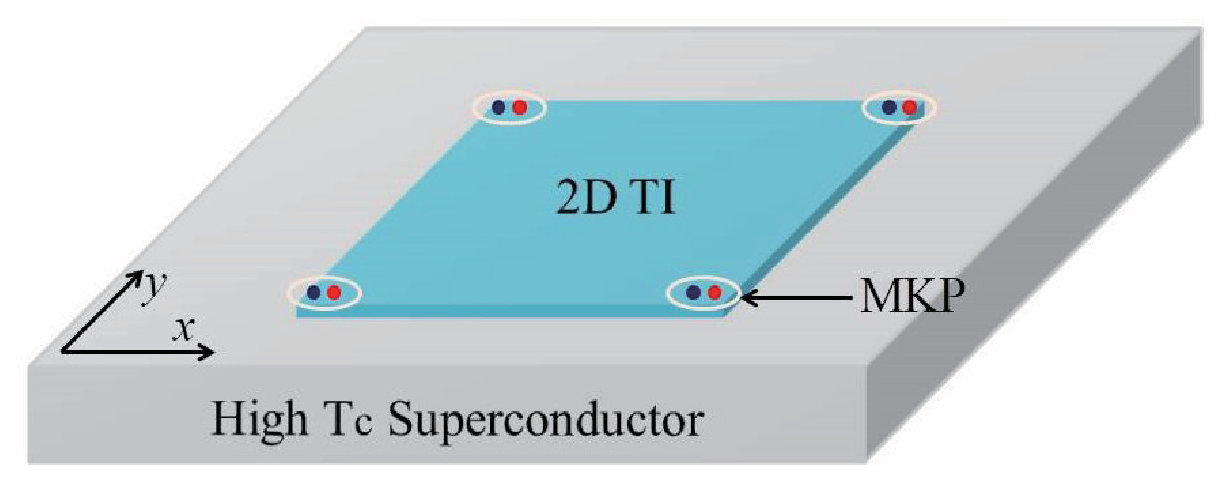
\includegraphics[scale=0.4]{pic/fig8}
\caption{示意图展示;一个2D拓扑绝缘体长在$d$-波或者$s_\pm$-波的高温超导体上,零能马约拉纳Kramers对(MKP)将会出现在2D拓扑绝缘体的角落。}\label{fig8}
\end{figure}
\end{frame}
%===============================================================
\begin{frame}{边界理论}
首先将哈密顿量(\ref{hoti2})在$\Gamma=(0,0)$处做低能展开,并保留到二阶
\begin{equation}
H(\mathbf{k})=(m+\frac{t_x}{2}k_x^2+\frac{t_y}{2}k_y^2)\sigma_z\tau_z+\lambda_xk_x\sigma_xs_z+\lambda_yk_y\sigma_y\tau_z-\frac{1}{2}(\Delta_xk_x^2+\Delta_yk_y^2)s_y\tau_y\label{hoti2e}
\end{equation}
取$x$方向在实空间$k_x\rightarrow-i\partial_x$,将哈密顿量(\ref{hoti2e})分解成两部分$H=H_0+H_p$
\begin{equation}
\begin{aligned}
H_0(-i\partial_x,k_y)&=(m-t_x\partial_x^2/2)\sigma_z\tau_z-i\lambda_x\sigma_xs_z\partial_x\\
H_p(-i\partial_x,k_y)&=\lambda_yk_y\sigma_y\tau_z+\frac{\Delta_y}{2}s_y\tau_y\partial_x^2
\end{aligned}
\end{equation}
在边界条件$\psi_\alpha(0)=\psi_\alpha(\infty)$下来求解$H_0\psi_\alpha(x)=E_\alpha\psi_\alpha(x)$可以得到四个零能解,其形式为
\begin{equation}
\psi_\alpha(x)=\mathcal{N}_x\sin(\kappa_1x)e^{-\kappa_2x}e^{ik_yy}\xi_\alpha
\end{equation}
\end{frame}
%------------------------------------
\begin{frame}{边界理论}
归一化系数为 $|\mathcal{N}_x|^2=4|\kappa_2(\kappa_1^2+\kappa_2^2)/\kappa_1^2|$。(符号简记,$\kappa_1=\sqrt{|(2m_x/t_x)|-(\lambda_x^2/t_x^2)}$,$ \kappa_2=(\lambda_x/t_x)$)。旋量部分 $\xi_\alpha$ 满足 $\sigma_ys_z\tau_z=-\xi_\alpha$,可以将旋量部分选取为
\begin{equation}
\begin{aligned}
\xi_1&=|\sigma_y=-1\rangle\otimes|\uparrow\rangle\otimes|\tau=+1\rangle\\
\xi_2&=|\sigma_y=+1\rangle\otimes|\downarrow\rangle\otimes|\tau=+1\rangle\\
\xi_3&=|\sigma_y=+1\rangle\otimes|\uparrow\rangle\otimes|\tau=-1\rangle\\
\xi_4&=|\sigma_y=-1\rangle\otimes|\downarrow\rangle\otimes|\tau=-1\rangle
\end{aligned}
\end{equation}
在这个基矢的选取下,微扰部分$H_p$计算为
\begin{equation}
H_{\uppercase\expandafter{\romannumeral1},\alpha\beta}(k_y)=\int_{0}^{\infty}dx\psi^*_\alpha(x)H_p(-i\partial_x,k_y)\psi_\beta(x);
\end{equation}
最后得到有效哈密顿量为
\begin{equation}
H_{\uppercase\expandafter{\romannumeral1}}(k_y)=-A_yk_ys_z+M_{\uppercase\expandafter{\romannumeral1}}s_y\tau_y
\end{equation}	
\end{frame}
%-------------------------------------------------------
\begin{frame}{边界理论}
\begin{equation}
M_{\uppercase\expandafter{\romannumeral1}}=\frac{\Delta_x}{2}\int_{0}^{\infty}dx\psi_\alpha^*(x)\partial_x^2\psi_\alpha(x)=\Delta_x\frac{m}{t_x}
\end{equation}
其它三个边界上的有效哈密顿量也可以通过相似方式求解得到,结果为
\begin{equation}
\begin{aligned}
H_{\uppercase\expandafter{\romannumeral1}}&=-A_yk_ys_z+M_{\uppercase\expandafter{\romannumeral1}}s_y\tau_y\\
H_{\uppercase\expandafter{\romannumeral2}}&=A_xk_xs_z+M_{\uppercase\expandafter{\romannumeral2}}s_y\tau_y\\
H_{\uppercase\expandafter{\romannumeral3}}&=A_yk_ys_z+M_{\uppercase\expandafter{\romannumeral3}}s_y\tau_y\\
H_{\uppercase\expandafter{\romannumeral4}}&=-A_xk_xs_z+M_{\uppercase\expandafter{\romannumeral4}}s_y\tau_y\\\label{edge1}
\end{aligned}
\end{equation}
每条边界上的质量项满足$M_{\uppercase\expandafter{\romannumeral2}}=M_{\uppercase\expandafter{\romannumeral4}}=\Delta_ym/t_y$,$M_{\uppercase\expandafter{\romannumeral1}}=M_{\uppercase\expandafter{\romannumeral3}}=\Delta_xm/t_x$。

\end{frame}
%--------------------------------------------------------------
\begin{frame}{边界理论}
	这里以逆时针方向为绕行正方向,可以将低能边界理论整理为
	\begin{equation}
	H_{\mathrm{edge}}=-iA(l)s_z\partial_l+M(l)s_y\tau_y\label{edge2}
	\end{equation}
这里的动能系数$A(l)$与Dirac质量项$M(l)$都是阶跃函数:$A(l)=A_y,A_x,A_y,A_x$,$M(l)=\Delta_dm/t_x,-\Delta_dm/t_y,\Delta_dm/t_x,-\Delta_dm/t_y$($l=\mathrm{\uppercase\expandafter{\romannumeral1},\uppercase\expandafter{\romannumeral2},\uppercase\expandafter{\romannumeral3},\uppercase\expandafter{\romannumeral4}}$)。

从这里可以看出,在系统的每个角落,系数$A_{x,y}$并不会改变符号,但是Dirac质量项$M_(l)$因为$d$-波配对$\Delta_x=-\Delta_y$的原因,在每个角落的位置都会反号,从而在每个角落处产生一个质量畴壁,形成类似于Jackiw-Rebbi零能模的束缚态。例如在边界($\mathrm{\uppercase\expandafter{\romannumeral1}}$)与($\mathrm{\uppercase\expandafter{\romannumeral2}}$)形成的角落中,零能束缚态波函数为
\begin{equation}
|\Psi^\pm_{\mathrm{MKP}}\rangle\sim e^{-\int^ldl^{'}M(l^{'})/A(l^{'})}|s_x=\tau_y=1\rangle
\end{equation}
由于哈密顿量满足时间反演不变,它保证了这两个零能态之间不会相互耦合并产生能隙。
\end{frame}
%---------------------------------------------------------------
\begin{frame}{高阶拓扑超导体}
\begin{equation}
\begin{aligned}
H^{\mathrm{BdG}}(\mathbf{k})&=(h^{\mathrm{TI}}(\mathbf{k})-\mu)\tau_z+\Delta(\mathbf{k})\tau_x\\
h^{\mathrm{TI}}(\mathbf{k})&=\left[2t(\cos k_x-\cos k_y)+4t_1\cos k_x\cos k_y\right]\sigma_z+2\lambda(\sin k_xs_y-\sin k_ys_x)\sigma_x\\
\Delta(\mathbf{k})&=\Delta_0+2\Delta_1(\cos k_x+\cos k_y)\label{hosc2}
\end{aligned}
\end{equation}
\begin{figure}[h]
\centering
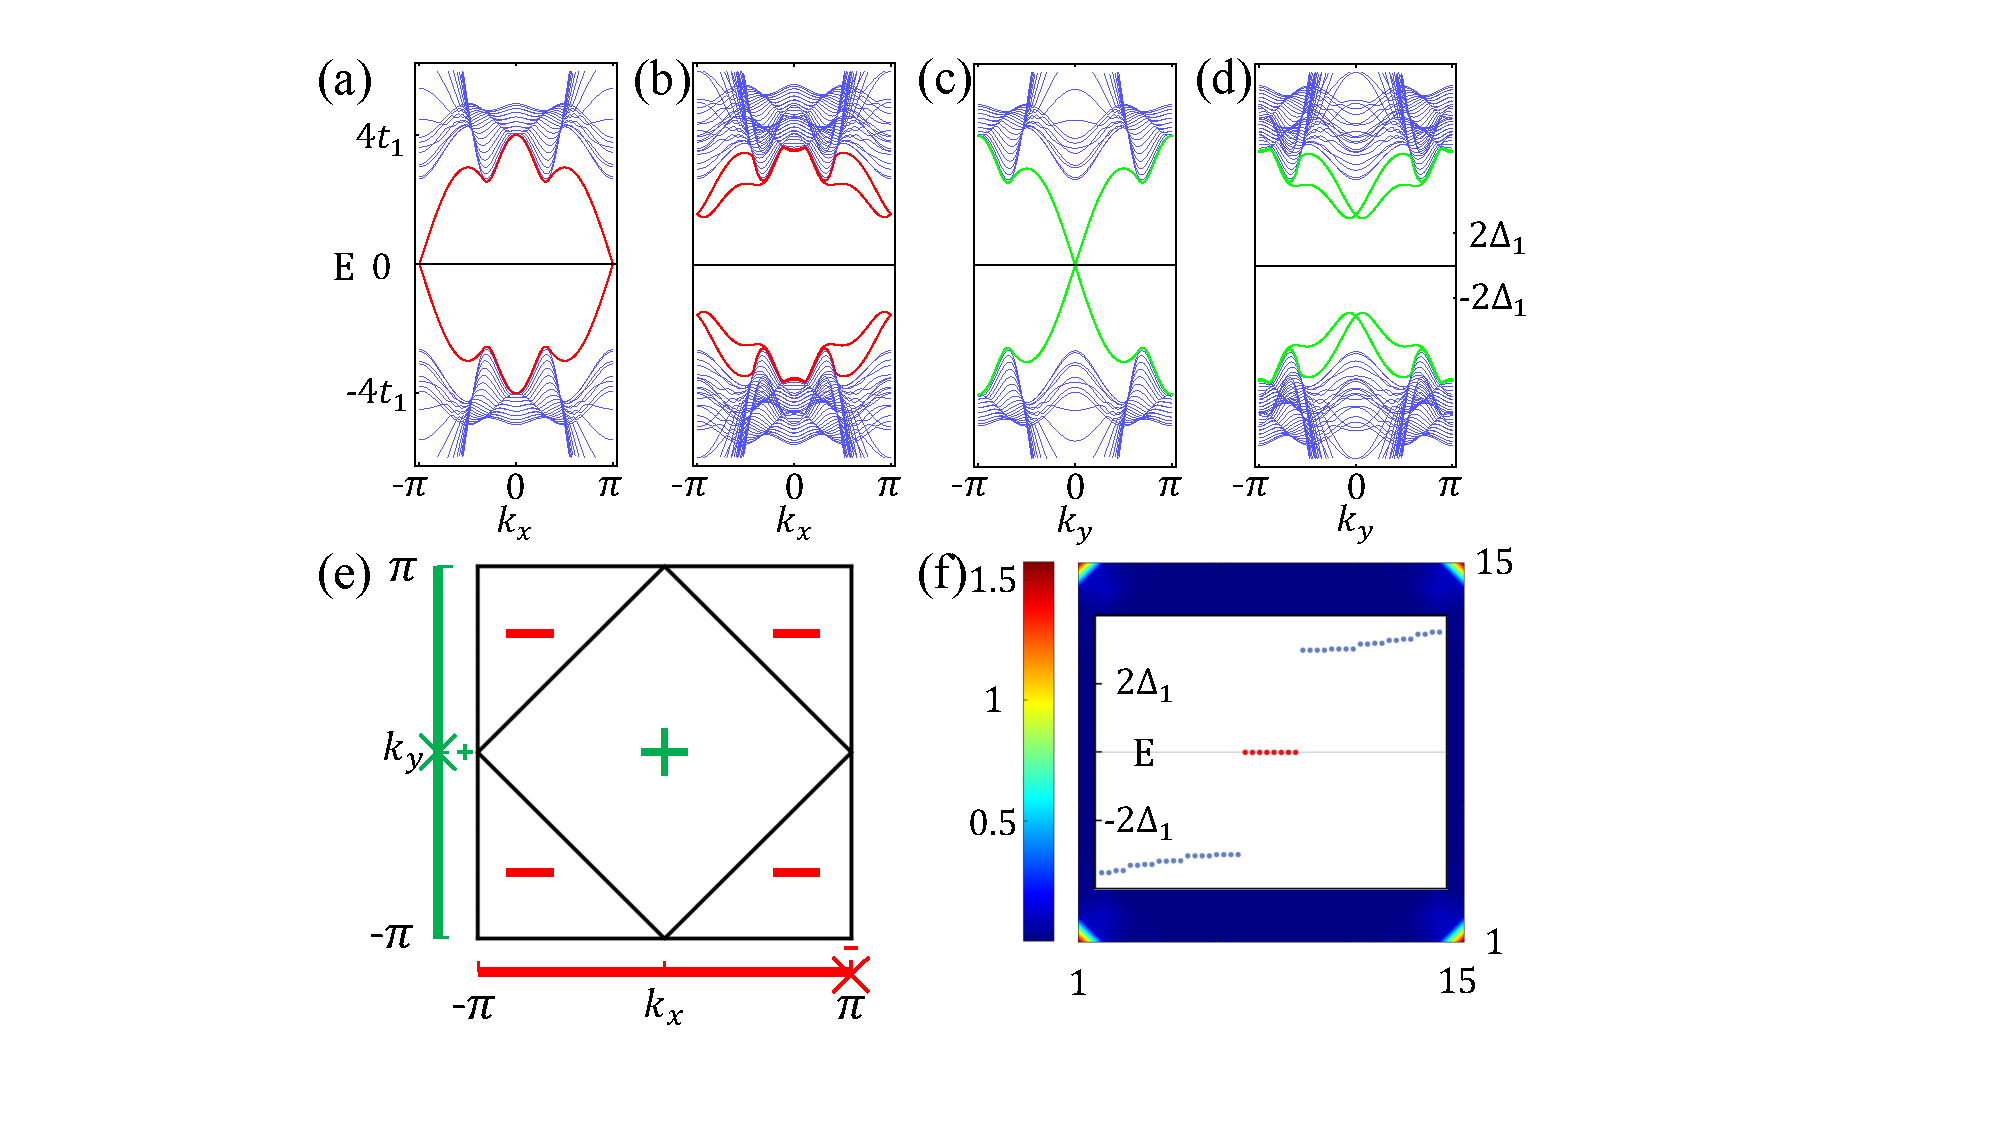
\includegraphics[scale=0.3]{pic/fig13}\label{fig12}
\end{figure}
\end{frame}
%--------------------------------------------------------------
\begin{frame}{高阶拓扑超导体}
\begin{equation}
\begin{aligned}
H(\mathbf{k})&=2\lambda_x\sin k_x\sigma_xs_z\tau_z+2\lambda_y\sin k_y\sigma_y\tau_z+(\xi_k\sigma_z-\mu)\tau_z+\Delta_0\tau_x+{\bf h\cdot s}\\
\xi_k&=\epsilon_0-2t_x\cos k_x-2t_y\cos k_y\label{ze1}
\end{aligned}
\end{equation}
\begin{figure}[h]
	\centering
	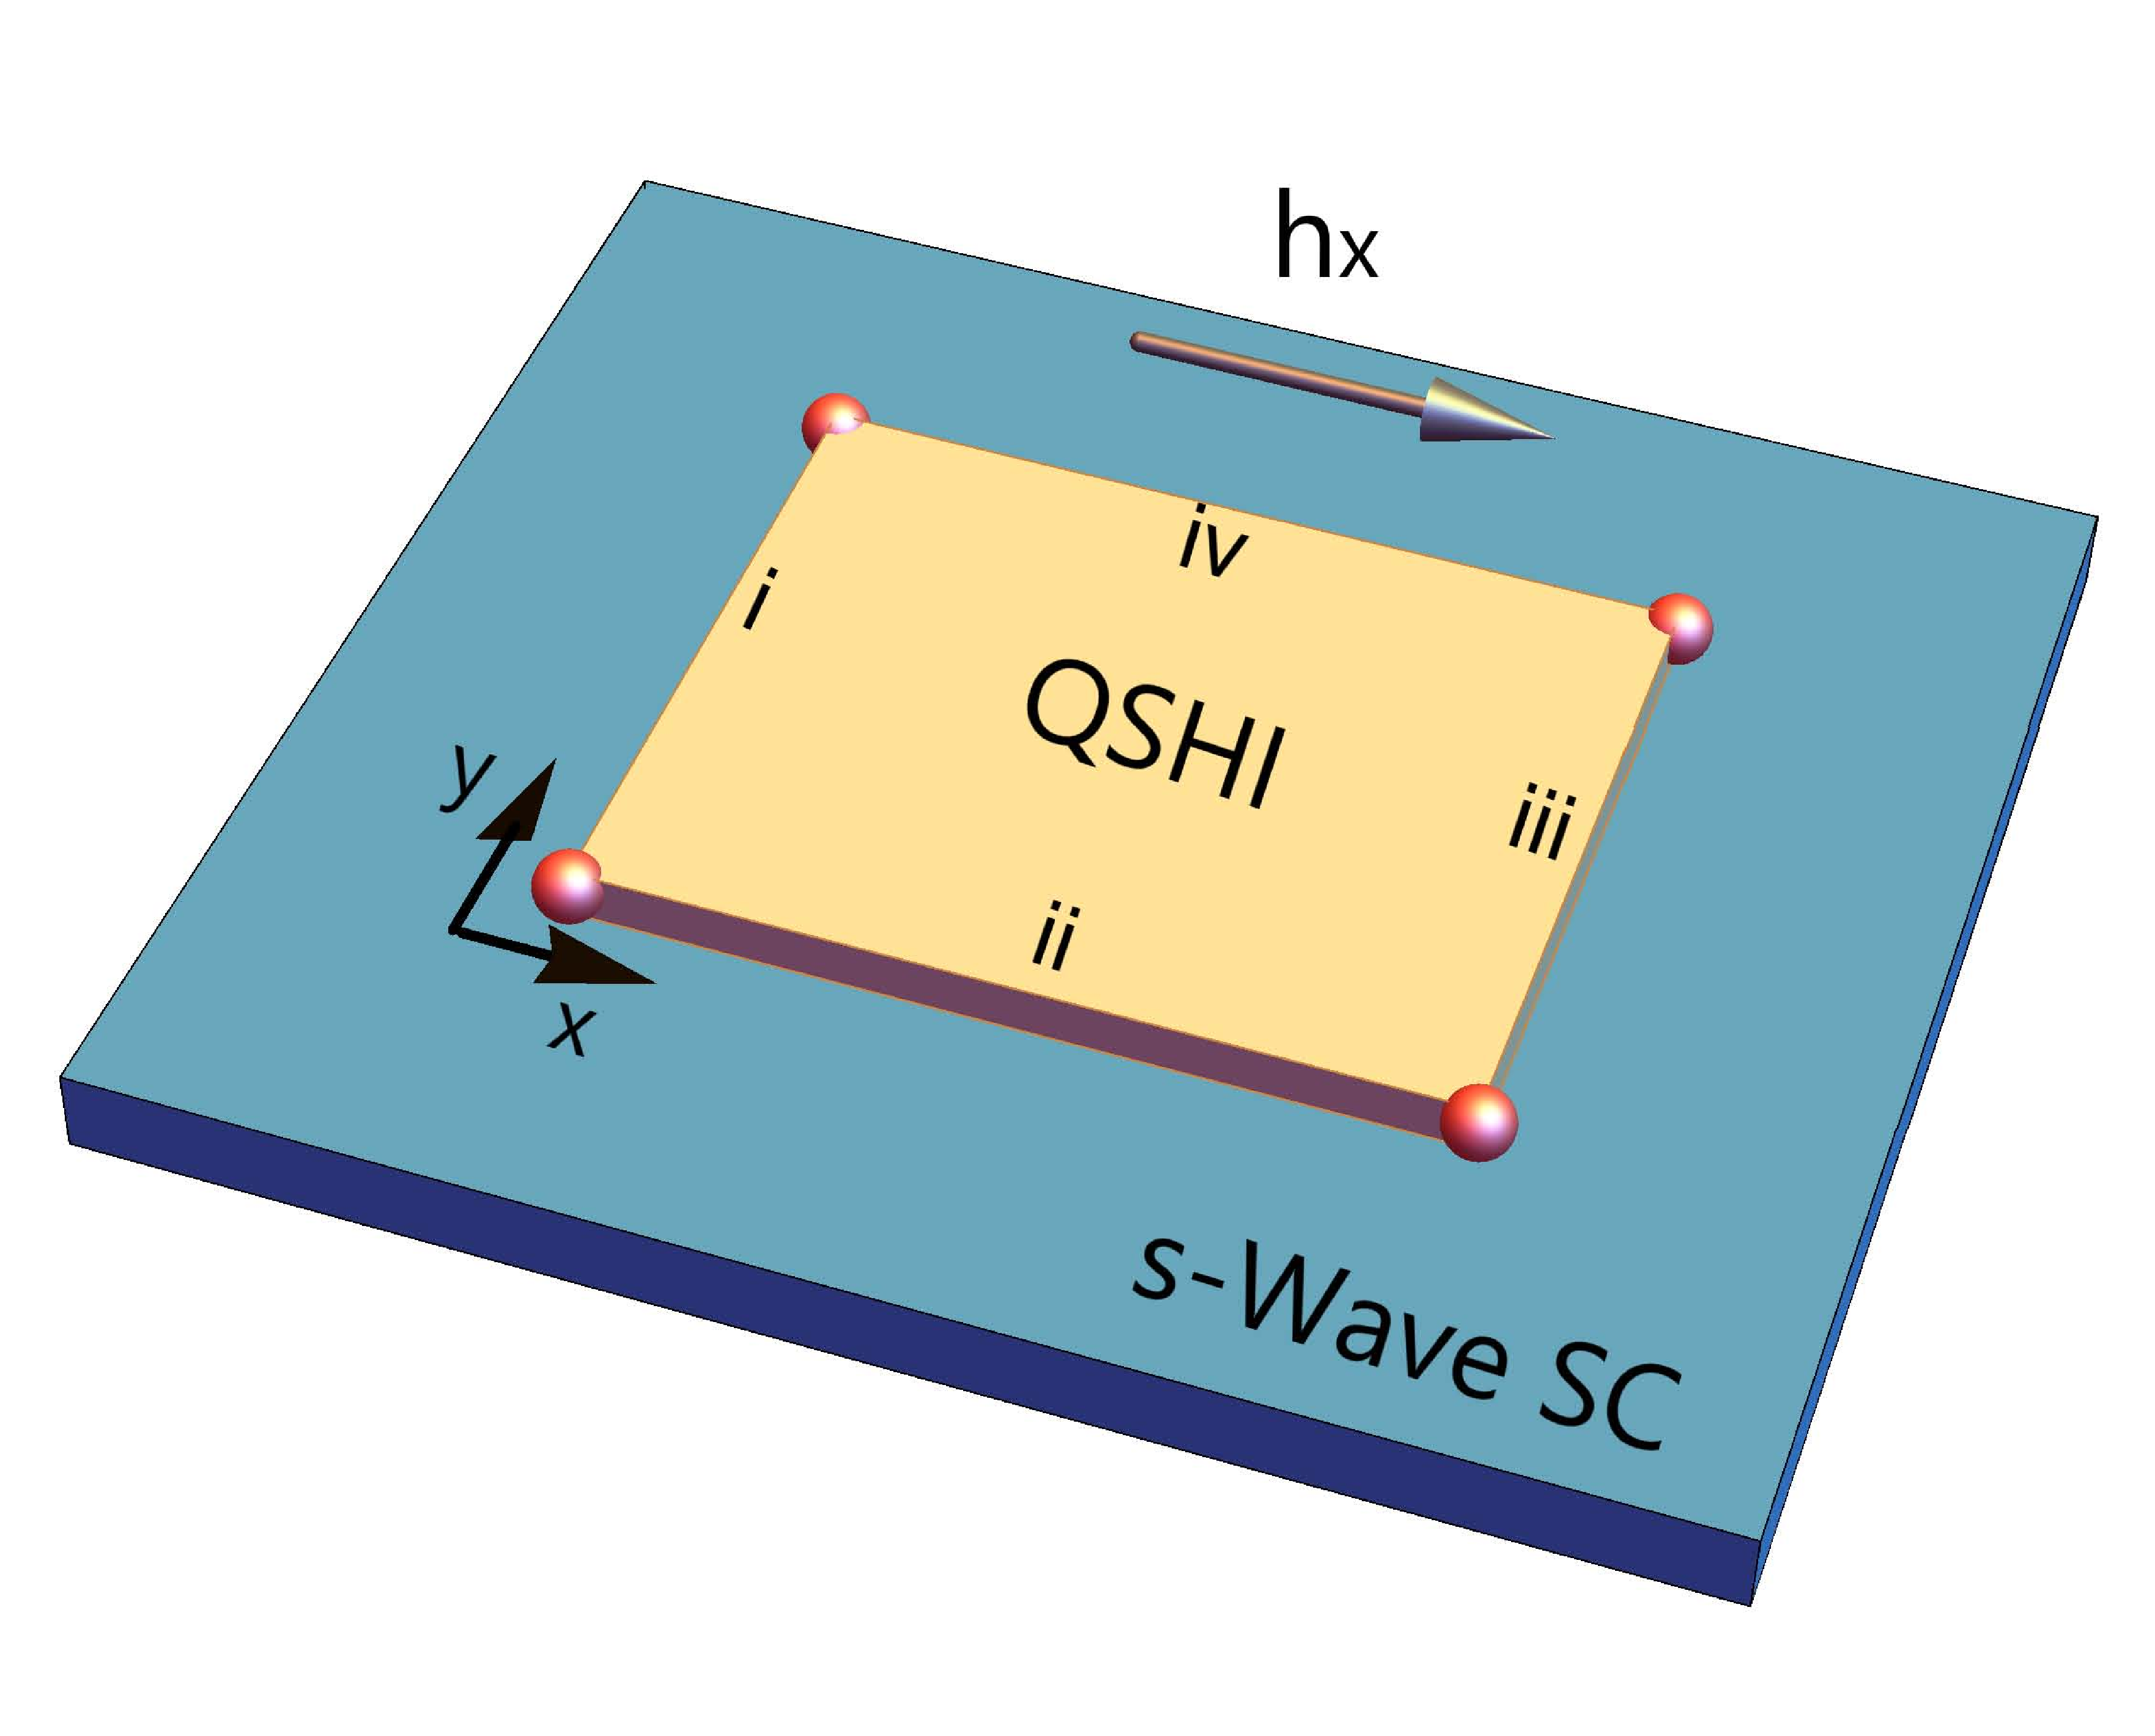
\includegraphics[scale=0.1]{pic/fig14.pdf}
	\caption{量子自旋霍尔效应与$s$-波超导构成异质结,并在面内存在一个各项异性的磁场,马约拉纳零能模出现在系统的四个拐角处。}\label{fig13}
\end{figure}
\end{frame}
%------------------------------------------------
\begin{frame}{近邻效应}
\begin{figure}[h]
\centering
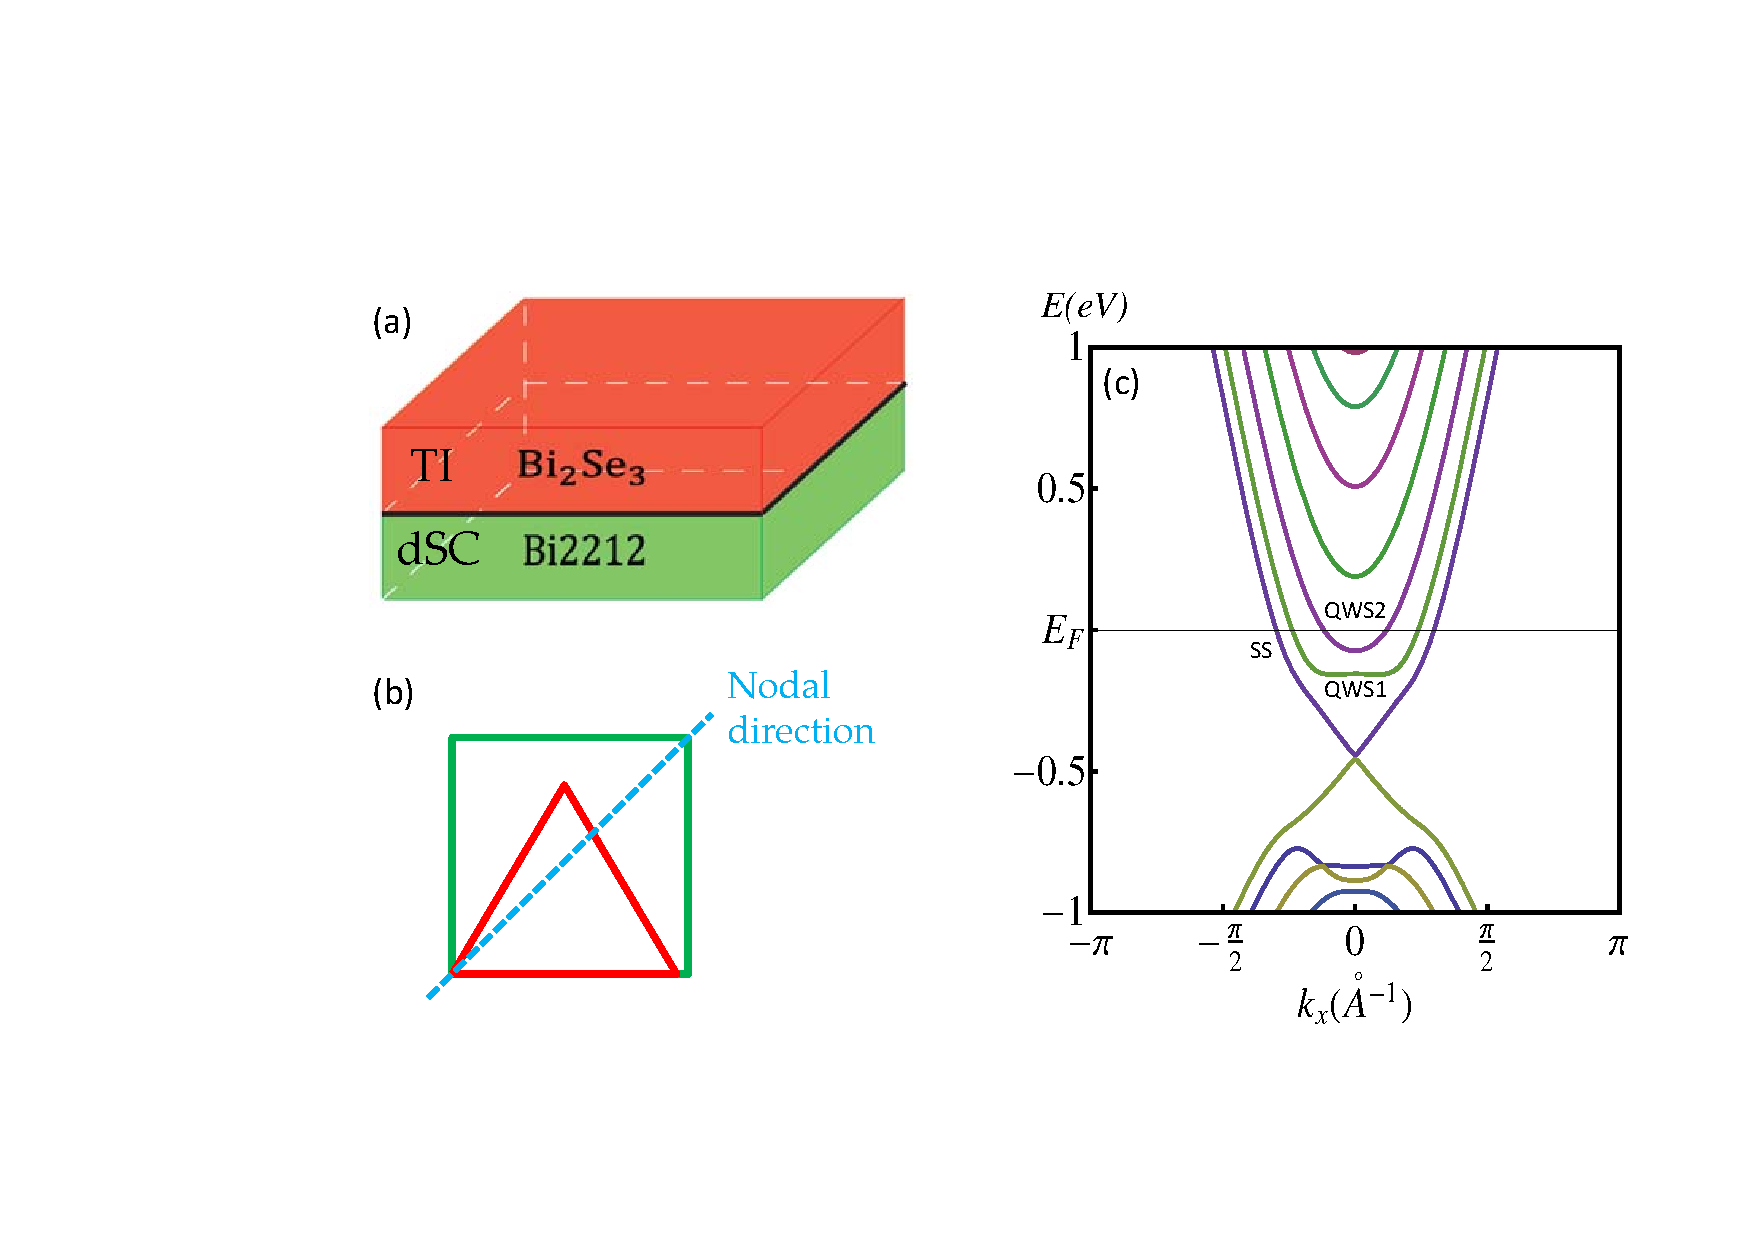
\includegraphics[scale=0.48]{pic/fig15.pdf}
\caption{(a)拓扑绝缘体/高温超导体异质结。(b)Bi$_2$Se$_3$与BSCCO的相对晶格取向,沿着超导配对节线方向,体系波坏了$90^\circ$旋转和反射对称。(c)拓扑绝缘体Bi$_2$Se$_3$的能带结构}\label{fig14}
\end{figure}
\end{frame}
%===============================================================
\section{基本理论}
\begin{frame}{微观模型}
\begin{equation}
H=H_\mathrm{TI}+H_\mathrm{SC}+H_\mathrm{I}\label{ham}
\end{equation}
\begin{equation}
\begin{aligned}
H_{TI} =\sum_{{\bf k}}C_{{\bf k}}^\dagger (h_\mathbf{k}\sigma_3s_0+2\lambda_{0}\sin k_x\sigma_1s_3+2\lambda_0\sin k_y\sigma_2 s_0)C_{{\bf k}},
\end{aligned}
\end{equation}
\begin{equation}
H_{SC}=\sum_{{\bf k}\sigma}\varepsilon_{\bf k}d^\dagger_{{\bf k}\sigma}d_{{\bf k}\sigma}+\sum_{{\bf k}}\Delta_{\bf k}(d^\dagger_{{\bf k}\uparrow}d^\dagger_{{-\bf k}\downarrow}+h.c.),
\end{equation}
\begin{equation}
{\color{blue}H_{I}=-t_\perp \sum_{{\bf k}\tau\sigma}(c_{{\bf k}\tau\sigma}^\dagger d_{{\bf k}\sigma}+h.c.).}
\end{equation}
这里$h_\mathbf{k}=h_0-2t(\cos k_x+\cos k_y)$,$\varepsilon_{\bf k}=-2t(\cos k_x+\cos k_y)-\mu$.
整个的哈密顿量可以被写成矩阵形式。在动量空间中它是一个$12\times 12$的矩阵$\hat{M}$,$H=\sum_{\mathbf{k}}\Psi_\mathbf{k}^\dagger\hat{M}\Psi_\mathbf{k}$
\end{frame}
%=======================================================
\section{计算结果}
\begin{frame}{谱函数}
	\begin{equation}
	G_{ij}(E)=\sum_n\frac{u_{in}u^{*}_{jn}}{E-E_n+i\Gamma}.
	\end{equation}
	这里$u_{in}$ 和 $E_n$分别代表着矩阵的本征矢量和本征值。在动量空间中,2D拓扑绝缘体层的谱函数可以通过格林函数计算
	\begin{equation}
	A({\bf k},E)=-\frac{1}{\pi}\sum^4_{p=1}\mathrm{Im} G_{pp}({\bf k},E).
	\end{equation}
\begin{figure}[h]
	\centering
	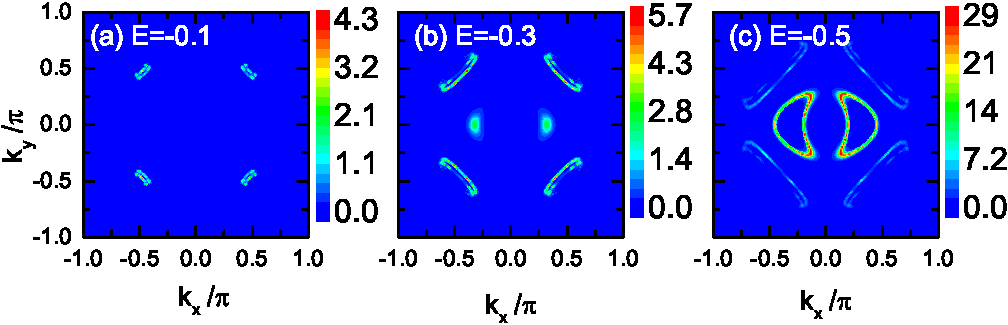
\includegraphics[scale=0.5]{pic/fig17.pdf}
	\caption{2D拓扑绝缘体层谱函数强度分布。(a)$E=-0.1$,(b)$E=-0.3$,(c)$E=-0.5$}\label{fig16}
\end{figure}
\end{frame}
%--------------------------------------------
\begin{frame}{边界态}
\begin{equation}
C^\dagger_\mathbf{k}=\frac{1}{\sqrt{N}}\sum_\mathbf{r}e^{i\mathbf{r}\cdot\mathbf{k}}C^\dagger_\mathbf{r}\qquad C^\dagger_\mathbf{r}=\frac{1}{\sqrt{N}}\sum_\mathbf{k}e^{-i\mathbf{r}\cdot\mathbf{k}}C^\dagger_\mathbf{r}
\end{equation}
\begin{figure}
\centering
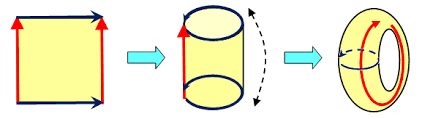
\includegraphics[scale=0.6]{pic/fig16}
\caption{圆柱形结构示意图}\label{fig15}
\end{figure}
\end{frame}
%-----------------------------------------------
\begin{frame}{边界态}
\begin{figure}[h]
	\centering
	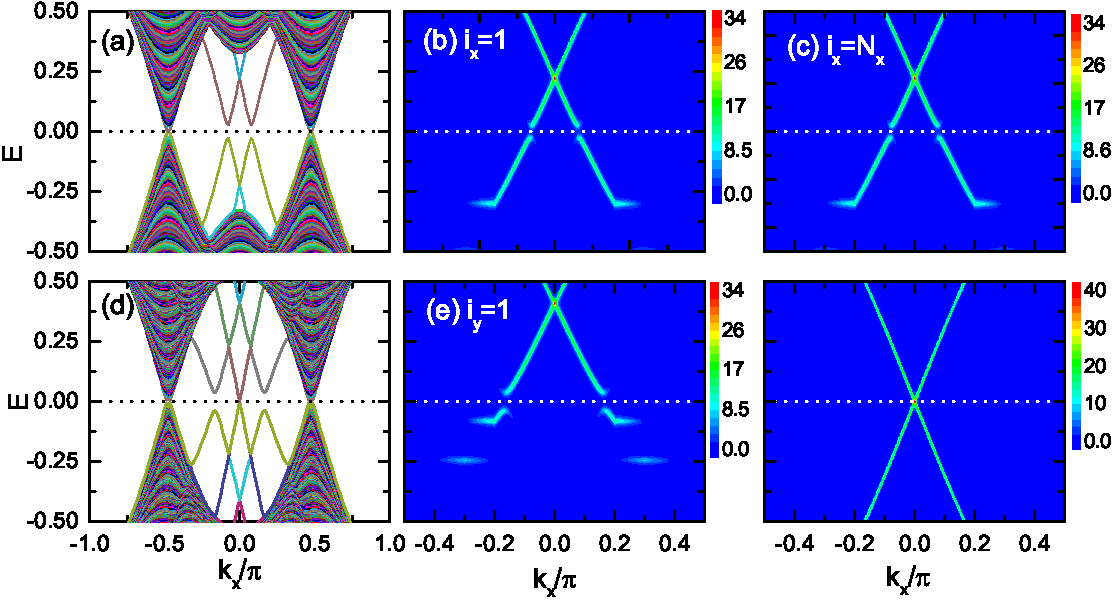
\includegraphics[scale=0.5]{pic/fig18.pdf}
	\caption{考虑圆柱形结构的数值计算结果。(a)沿$x$方向开边界时哈密顿量本征值,(b)$i_x=1$边界处的谱函数,(c)$i_x=N_x$边界处的谱函数,(d)沿$y$方向开边界时哈密顿量本征值,(b)$i_y=1$边界处的谱函数,(c)$i_y=N_y$边界处的谱函数}\label{fig17}
\end{figure}
\end{frame}
%-----------------------------------------------
\begin{frame}{局域电子态密度}
\begin{equation}
\rho_i(E)=-\frac{1}{\pi}\sum^4_{p=1}\mathrm{Im} G_{m+p,m+p}(E).
\end{equation}
\begin{figure}[h]
\centering
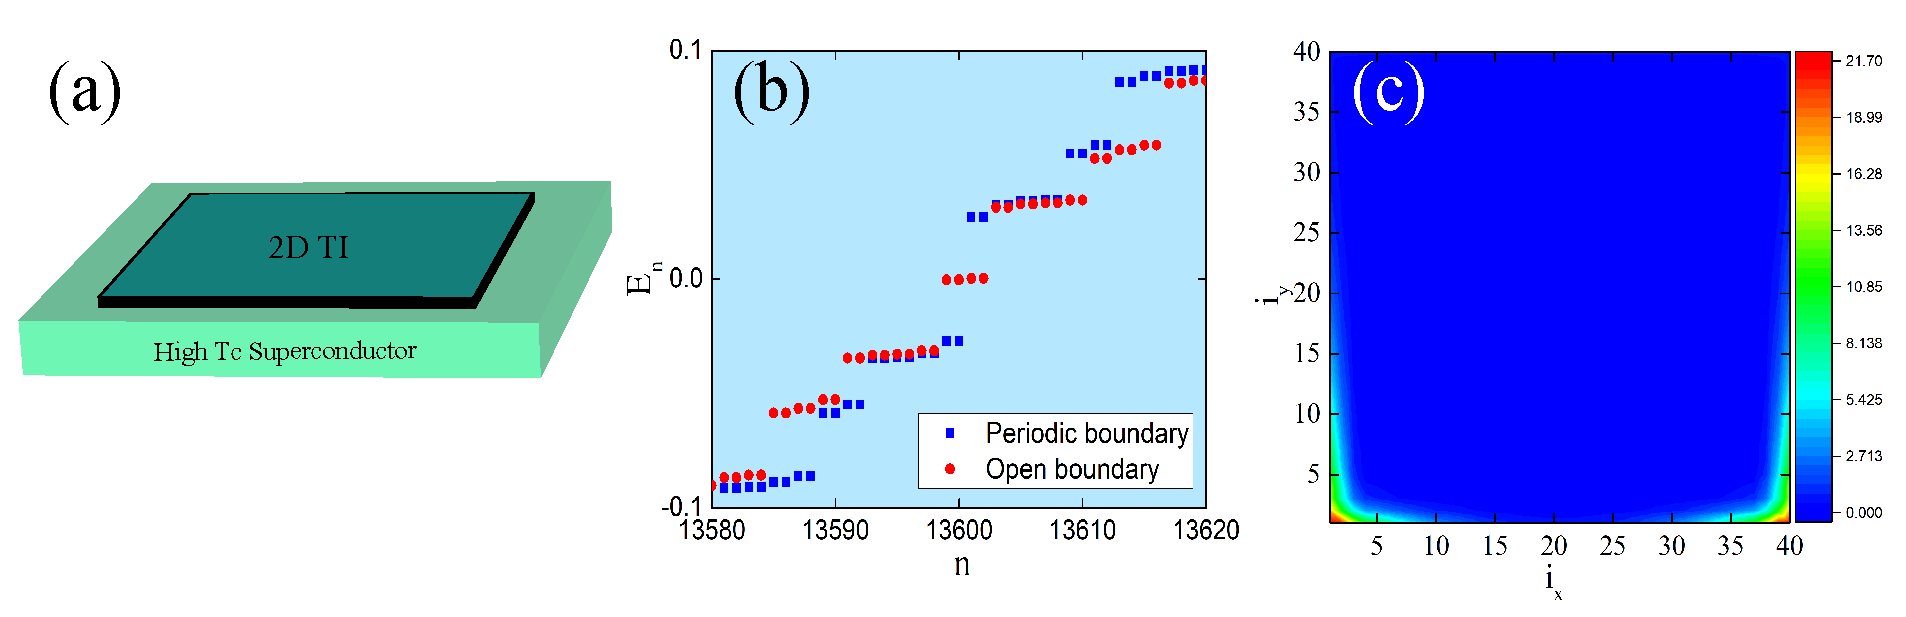
\includegraphics[scale=0.4]{pic/fig19}
\caption{(a)2D拓扑绝缘体生长在$d$-波高温超导体上,(b)实空间哈密顿量本征值(c)2D拓扑绝缘体实空间中零能态电子局域态密度}\label{fig18}
\end{figure}
\end{frame}
%----------------------------------------------
\begin{frame}{动量空间序参量}
	\begin{equation}
	\Delta_\tau({\bf k})=\langle c^\dagger_{{\bf k}\tau\uparrow}c^\dagger_{-{\bf k}\tau\downarrow}\rangle=\sum_n{u^{*}_{\tau,n}({\bf k})u_{\tau+6,n}({\bf k})}f(E_n),
	\end{equation}
\begin{equation}
\Delta_s(\mathbf{k})=\frac{1}{2}\left[\Delta_1(\mathbf{k})+\Delta_1(\mathbf{-k})\right]\qquad
\Delta_t(\mathbf{k})=\frac{1}{2}\left[\Delta_1(\mathbf{k})-\Delta_1(\mathbf{-k})\right]
\end{equation}
\begin{figure}[h]
\centering
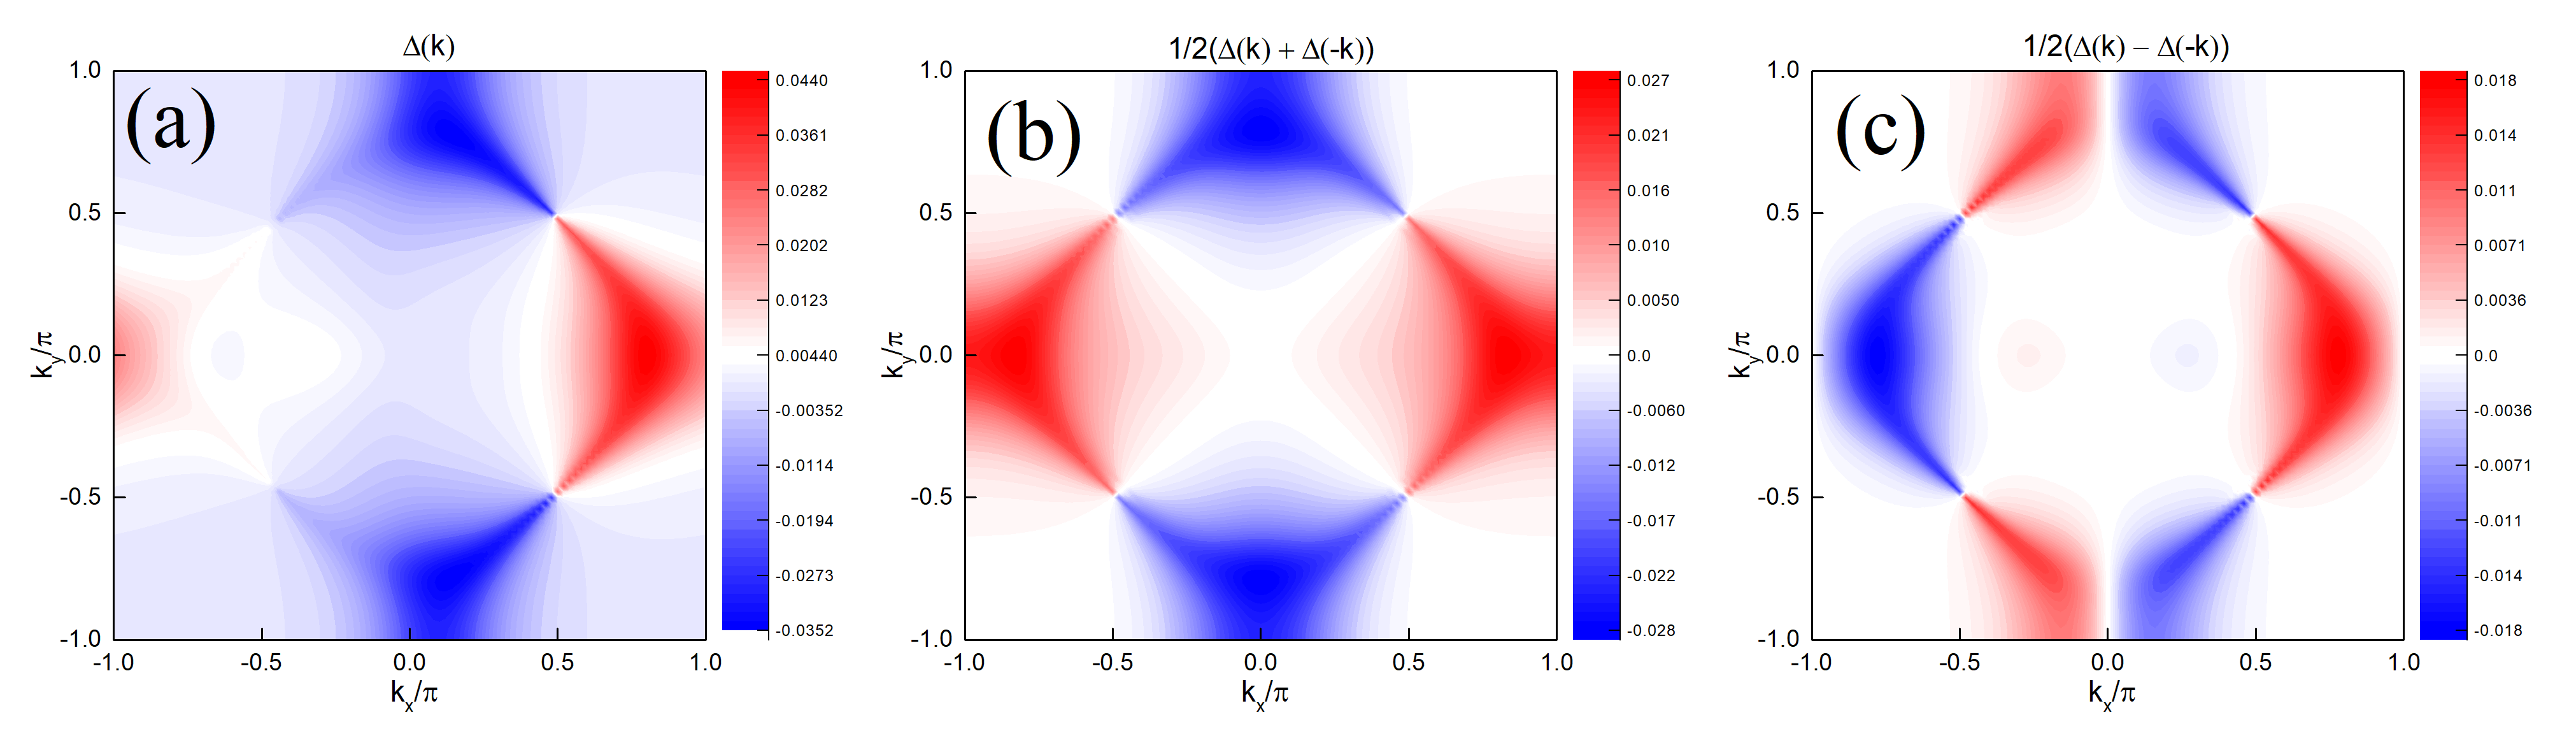
\includegraphics[scale=0.13]{pic/fig20}
\caption{(a)轨道1的超导序参量(b)轨道1单重态通道的序参量(c)轨道1三重态通道的序参量}\label{fig19}
\end{figure}
\end{frame}
%-----------------------------------------------
\begin{frame}{实空间序参量}
\begin{equation}
\Delta^\tau_{ij}=\sum_nu^{*}_{h(i),n}u_{h(j)+6,n}f(E_n),
\end{equation}
\begin{equation}
\Delta^\tau_i=\mid \Delta^\tau_{i,i+\hat{x}}+\Delta^\tau_{i,i-\hat{x}}
-\Delta^\tau_{i,i+\hat{y}}-\Delta^\tau_{i,i-\hat{y}}\mid.
\end{equation}
在系统的边界上,$\Delta_i^\tau$表示为
\begin{equation}
\Delta^\tau_i=\mid 2(\Delta^\tau_{i,i+\hat{\alpha}}+\Delta^\tau_{i,i-\hat{\alpha}}) \mid  \qquad (\alpha=x,y).
\end{equation}
\begin{figure}[h]
\centering
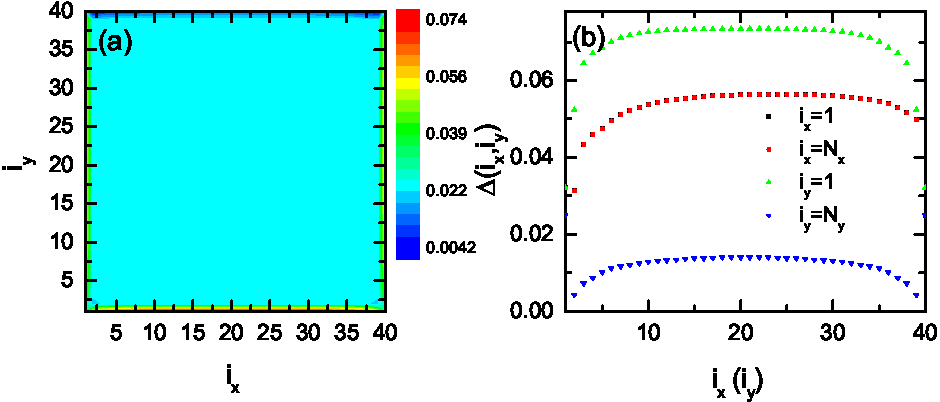
\includegraphics[scale=0.5]{pic/fig21}
\caption{(a)2D拓扑绝缘体轨道1实空间中的$d$-波序参量(b)实空间四条边界上的$d$-波序参量分布}\label{fig20}
\end{figure}
\end{frame}
%===============================================================
\begin{frame}{反常格林函数}
对于2D拓扑绝缘体,其轨道$\tau$的有效配对可以由反常格林函数$F_\tau(\mathbf{k},\omega)=\langle\langle c^\dagger_{\mathbf{k}\tau\uparrow}|c^\dagger_{\mathbf{-k}\tau\downarrow}\rangle\rangle$
\begin{equation}
F_\tau(\mathbf{k},\omega)=\sum_n\frac{u^{*}_{\tau,n}(\mathbf{k})u_{\tau+6,n}(\mathbf{k})}{\omega-E_n+i\Gamma}\label{af1}
\end{equation}
同样的,他可以解析的通过下面的运动方程来求解
\begin{equation}
\omega\langle\langle A|B\rangle\rangle=\langle\left[A,B\right]_{+}\rangle+\langle\langle\left[A,H\right]|B\rangle\rangle\label{gf11}
\end{equation}
\begin{equation}
H=H_\mathrm{TI}+H_\mathrm{SC}+H_\mathrm{I}\label{ham}
\end{equation}
先做一些简化的记号$x_1=\langle\langle c_{{\bf k}1\uparrow}^\dagger|c_{-{\bf k}1\downarrow}^\dagger\rangle\rangle_\omega$,
$x_2 = \langle\langle c_{{\bf k}2\uparrow}^\dagger|c_{-{\bf k}1\downarrow}^\dagger\rangle\rangle_\omega$,
$x_3 = \langle\langle d_{{\bf k}\uparrow}^\dagger|c_{-{\bf k}1\downarrow}^\dagger\rangle\rangle_\omega$,
$x_4 = \langle\langle d_{-{\bf k}\downarrow}|c_{-{\bf k}1\downarrow}^\dagger\rangle\rangle_\omega$,
$x_5 = \langle\langle c_{-{\bf k}1\downarrow}|c_{-{\bf k}1\downarrow}^\dagger\rangle\rangle_\omega$,
$x_6 = \langle\langle c_{-{\bf k}2\downarrow}|c_{-{\bf k}1\downarrow}^\dagger\rangle\rangle_\omega$
\end{frame}
%------------------------------------------------------
\begin{frame}{反常格林函数}
\begin{subequations}
	\begin{eqnarray}
	ax_1&=&fx_2+t_\perp x_3
	\\
	bx_2&=&ex_1+t_\perp x_3
	\\
	cx_3&=&gx_4+t_\perp (x_1+x_2)
	\\
	dx_4&=&gx_3-t_\perp (x_5+x_6)
	\\
	bx_5&=&1-fx_6-t_\perp x_4
	\\
	ax_6&=&-ex_5-t_\perp x_4,\label{eom2}
	\end{eqnarray}
\end{subequations}
这里 $a=\omega-h_{\bf k}$, $b=\omega + h_{\bf k}$, $c=\omega-\varepsilon_{\bf k}$,
$d=\omega+\varepsilon_{\bf k}$, $e=2\lambda_0\sin(k_x)-2i \lambda_0\sin(k_y)$, $f=2\lambda_0\sin(k_x) + 2i\lambda_0\sin(k_y)$,
并且令 $g = \Delta_{\bf k}$.

\begin{equation}
\langle\langle c_{{\bf k}1\uparrow}^\dagger|c_{-{\bf k}1\downarrow}^\dagger\rangle\rangle=\frac{\Delta_{\bf k} t_\perp ^2 (a-e) (b+f)}{\Omega}=\frac{\Delta_{\bf k}t_\perp^2(C_{even}+C_{odd})}{\Omega},\label{anlyagf}
\end{equation} $C_{even}=\omega^2-h^2_{\bf{k}}-4\lambda_0[\sin^2(k_x)+\sin^2(k_y)]$, $C_{odd}=4\omega\lambda i\sin(k_y)-4h_{\mathbf{k}}\lambda_0\sin(k_x)$
\end{frame}
%-----------------------------------------------------------
\begin{frame}{反常格林函数}
\begin{equation}
F_\tau({\bf k})=-\int_{-\infty}^0\mathrm{Im}F_\tau({\bf k},\omega)d\omega.
\end{equation}
\begin{equation}
\begin{aligned}
F_s({\bf k})&=1/2[F_1({\bf k})+F_1(-{\bf k})]\\
F_t({\bf k})&=1/2[F_1({\bf k})-F_1(-{\bf k})]
\end{aligned}
\end{equation}
\begin{figure}[h]
	\centering
	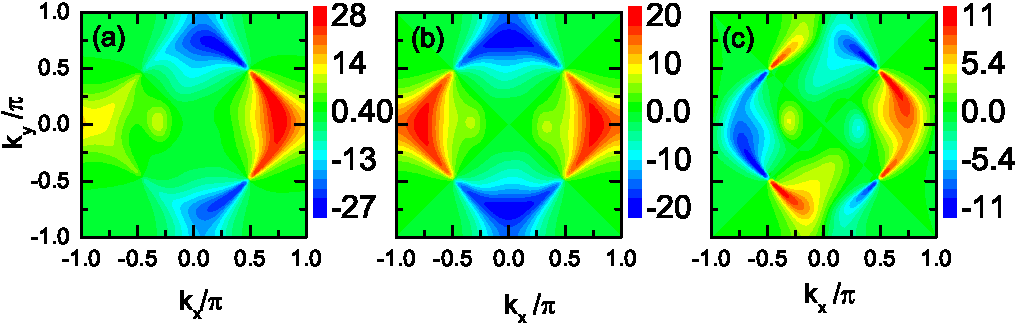
\includegraphics[scale=0.6]{pic/fig22}
	\caption{(a)反常格林函数计算轨道1的超导序参量(b)轨道1单重态通道的序参量(c)轨道1三重态通道的序参量}\label{fig21}
\end{figure}
\end{frame}
%------------------------------------------------------------
% Thank you page
\beamertemplateshadingbackground{structure.fg!50}{structure.fg}
\begin{frame}[plain]
	\vfill
	\centering
	{
		\centering \Huge \color{white} Thank you for your attention!\\[10pt]Questions?
	}
	\vfill
\end{frame}
%===============================================================
\end{document}
